\documentclass[11pt]{article}
\usepackage[pdftex]{graphicx}
\usepackage{fancyvrb, minted}
\usepackage[letterpaper, margin = 2.5cm]{geometry}
\usepackage[T1]{fontenc}
\usepackage{amsfonts, amssymb}
\usepackage{hyperref, url} 
\usepackage{fancyhdr}
\usepackage{tikz}
% \usetikzlibrary{arrows}
% \usetikzlibrary{automata}
\usepackage[fleqn]{nccmath}
\usepackage{enumitem}
% \usetikzlibrary{arrows.meta, shapes, positioning}

\thinmuskip=5mu

\fancypagestyle{firstpage}{
  \fancyhf{}
  \fancyhead[L]{
  Universidade Federal do Rio Grande do Sul
  \\ Programa de Pós-Graduação em Computação
  \\ AGL09018 - Inteligência Artificial Avançada
  \\ Professor André Grahl Pereira
  }
  \renewcommand{\headrulewidth}{0.4pt}
}

\begin{document}

\begin{titlepage}

    \thispagestyle{firstpage}
    \vspace*{1in}
    \begin{center}
      {\LARGE\bfseries List 3 \par}
      \vspace{0.2in}
      {\large Matheus Westhelle \par}
    \end{center}

\section*{Exercise 1}

\begin{enumerate}[label=(\alph*)]
\item Provide planning tasks in positive normal form with the following characteristics, or justify
why no such a task exists.
\begin{enumerate}[label=(\roman*)]
\item A task $\Pi_1$ that is unsolvable, but with $\Pi^{+}_1$ having an optimal plan length of 2. \par
\vspace{5mm}
Let $\Pi_1 = \langle \, V, I, O, \gamma \, \rangle$, where $V = \{ a, b, c \}$,
$I = \{ a \}$,
$\gamma = a \land b \land c$, and we have
the following operators $O$:
\begin{align*}
    O_1 &= \langle \, \,a, b, 1 \, \rangle \\
    O_2 &= \langle \, b, c \land \neg\,a, 1 \, \rangle
\end{align*}

This task is unsolvable, as it's not possible to reach $a \land b \land c$ due to the $\neg a$ delete
effect of operator $O_2$. We then define $\Pi_1^{+}$, which only differs from $\Pi_1$ on
the $O_2$ operator:

\begin{align*}
    O_2^{+} &= \langle \, b, c, 1 \, \rangle
\end{align*}

\noindent For task $\Pi_1^{+}$, we can sequentially apply $O_1^{+}$ and $O_2^{+}$, which gives us a solution of length 2.

\item A task $\Pi_2$ with optimal plan length of 2, but such that $\Pi_2^{+}$ is unsolvable.
\vspace{5mm}

No such task exists. The relaxation lemma states that if a plan $\pi$ leads to a goal state from
state $s$, then $\pi^{+}$ leads to a goal state from $s'$. If there is no plan $\pi^{+}$ that leads
to a goal state, as task $\Pi_2^{+}$ is unsolvable, by \textit{modus tollens}, this violates the relaxation lemma.

\item A task $\Pi_3$ with set of operators $O = \{o_1, o_2, o_3\}$ such that $\Pi_3^{+}$
has an optimal plan of length 4. \par
\vspace{5mm}
Let $\Pi_3 = \langle \, V, I, O, \gamma \, \rangle$ with $V = \{ r, s, t, u \}$, $I = \{ r \}$,
$\gamma = r \land s \land t \land u \land v$, and operators $O$:

\begin{align*}
    O_1 &= \langle \, r, s, 1 \, \rangle \\
    O_2 & = \langle \, s, t, 1 \, \rangle \\
    O_3 &= \langle \, t, u \land \neg \, t, 1 \, \rangle
\end{align*}

Task $\Pi_3$ has the optimal plan $\pi^{*} = \langle \, O_1, O_2, O_3, O_2 \, \rangle$.

\item An infinite family of planning tasks $P = \{ P_1, P_2, ... \}$ (e.g. the definition of $P_i$ is
parametrized by the value of integer parameter $i$) such that the optimal plan length of each task
$P_i$ increases with the value of $i$, but the optimal plan length of any $P_i^{+}$ is always 1. \par
\vspace{5mm}
Answer: Let a planning task $P$ be defined parametrically as $V_i = \{ v_1, v2 ..., v_{i1} \}$, $I_i = \{ v_1 \}$,
$\gamma = v_1 \land ... \land v_i$. We then define, for each task $P_i$, operators as such:

\begin{align*}
    & O_{1} = \langle \, v_1, v_2, 1 \, \rangle \\
    & O_{i} = \langle \, v_{i - 1}, v_i, 1 \, \rangle \\
    \omit\span\omit\hfil\vdots\hfil \\
    & O_{i+1} = \langle \, \top, \neg \, v_1 \land v_2, ..., v_i, 1  \, \rangle
\end{align*}

The last operator has a delete effect for the variable in the initial state, but contains all other
variables necessary for the goal, such that its relaxed counterpart $O_{i+1}^+$ is sufficient to form
a plan by itself ($\pi_i = \langle \, O_{i+1}^+ \, \rangle$) that reaches the goal from the initial state with length 1. For the original planning task, the optimal plan length grows as $i$
increases.

\end{enumerate}

\item Take the simple instance of the Visitall domain (from the International Planning Competition)
in directory visitall-untyped, and make sure you understand the problem.
What is the optimal solution value $h^{*}(I)$? \par
\vspace{5mm}

For this instance of the problem, the robot starts in the midpoint of a single row of five
rooms, and it must visit them all. For notation, we denote that the robot is at position $i$ using
$r_i$, and that position $i$ has been visited with $v_i$. In this instance, the domain of $i$ is
${0, 1, 2, 3, 4}$. In order to visit all rooms, the robot
has two optimal paths: it can either go all the way to the leftmost room $r_0$,
and then ``turn around'' and move until the rightmost position, $r_4$; or it can start by moving all the
way to the right, and then all the way to the left until $r_0$. The plans are:

\begin{align*}
\pi_1^{*} = \langle \, Move(r_2, r_1), Move(r_1, r_0), Move(r_0, r_1), Move(r_1, r_2), \\
Move(r_2, r_3), Move(r_3, r_4) \, \rangle
\end{align*}

And

\begin{align*}
\pi_2^{*} = \langle \, Move(r_2, r_3), Move(r_3, r_4), Move(r_4, r_3), Move(r_3, r_2), \\
Move(r_2, r_1), Move(r_1, r_0) \, \rangle
\end{align*}

Both plans have length 6. Thus, $h^{*}(I) = 6$. \par
\vspace{5mm}

What is the value of $h^{+}(I)$?\par
\vspace{5mm}
For the relaxed version of the task, we don't account for the fact the robot needs to backtrack,
as we don't consider the delete effects that remove him from the previous room at each movement.
Thus, we simply visit one room at a time, as long as it is adjacent to rooms the robot has already
visited. One optimal relaxed plan is:

\begin{align*}
    \pi^{+} = \langle \, Move(r_2, r_1), Move(r_1, r_0), Move(r_2, r_3), Move(r_3, r_4) \, \rangle
\end{align*}

Thus, we have $h^{+}(I) = 4$. \par
\vspace{5mm}

Draw the full Relaxed Task Graph corresponding to the instance, and label each node with the
final cost that results from (manually) applying the algorithm seen in class for computing $h^{max}$. What is the value of $h^{max}(I)$?
\vspace{5mm}

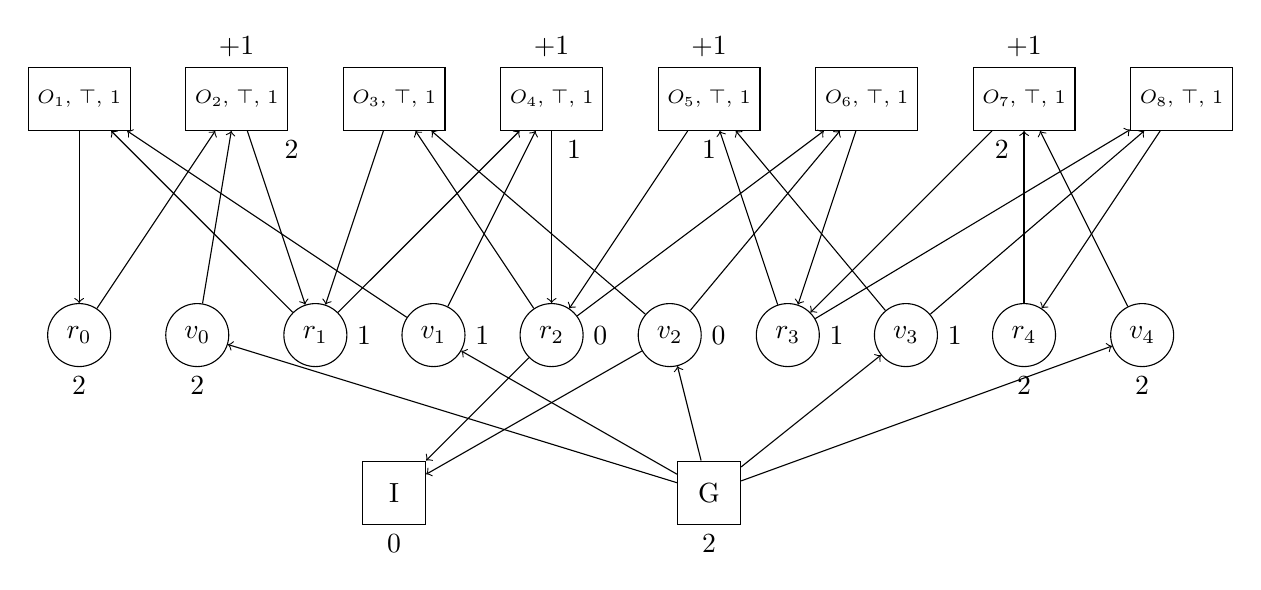
\begin{tikzpicture}[
        node distance=1.5cm and 1cm,
        mycirc/.style={draw, circle, minimum size=0.8cm}
        ]
    % Define styles
    \tikzstyle{square} = [draw, rectangle, minimum size=0.8cm]

    % Define operator nodes
    \node[square, font=\scriptsize] (O1) at (0, 6) {$O_1$, $\top$, 1};
    \node[square, font=\scriptsize, label=above:{+1}, label=-40:{2}] (O2) at (2, 6) {$O_2$, $\top$, 1};
    \node[square, font=\scriptsize] (O3) at (4, 6) {$O_3$, $\top$, 1};
    \node[square, font=\scriptsize, label=above:{+1}, label=-80:1] (O4) at (6, 6) {$O_4$, $\top$, 1};
    \node[square, font=\scriptsize, label=above:{+1}, label=below:{1}] (O5) at (8, 6) {$O_5$, $\top$, 1};
    \node[square, font=\scriptsize] (O6) at (10, 6) {$O_6$, $\top$, 1};
    \node[square, font=\scriptsize, label=above:{+1}, label=-100:{2}] (O7) at (12, 6) {$O_7$, $\top$, 1};
    \node[square, font=\scriptsize] (O8) at (14, 6) {$O_8$, $\top$, 1};

    % Define variable nodes
    \node[mycirc, label=below:{2}] (r0) at (0, 3) {$r_0$};
    \node[mycirc, label=below:{2}] (v0) at (1.5, 3) {$v_0$};
    \node[mycirc, label=right:{1}] (r1) at (3, 3) {$r_1$};
    \node[mycirc, label=right:{1}] (v1) at (4.5, 3) {$v_1$};
    \node[mycirc, label=right:{0}] (r2) at (6, 3) {$r_2$};
    \node[mycirc, label=right:{0}] (v2) at (7.5, 3) {$v_2$};
    \node[mycirc, label=right:{1}] (r3) at (9, 3) {$r_3$};
    \node[mycirc, label=right:{1}] (v3) at (10.5, 3) {$v_3$};
    \node[mycirc, label=below:{2}] (r4) at (12, 3) {$r_4$};
    \node[mycirc, label=below:{2}] (v4) at (13.5, 3) {$v_4$};

    % Define initial state and goal nodes
    \node[square, label=below:{0}] (I) at (4, 1) {I};
    \node[square, label=below:{2}] (G) at (8, 1) {G};

    % Draw edges from bottom from variable nodes to initial state
    \draw[->] (r2) -- (I);
    \draw[->] (v2) -- (I);

    % Draw edges from operator nodes to precondition nodes
    \draw[->] (O1) -- (r0);
    \draw[->] (O2) -- (r1);
    \draw[->] (O3) -- (r1);
    \draw[->] (O4) -- (r2);
    \draw[->] (O5) -- (r2);
    \draw[->] (O6) -- (r3);
    \draw[->] (O7) -- (r3);
    \draw[->] (O8) -- (r4);

    % Draw the edges from effect nodes to operator nodes
    \draw[->] (r1) -- (O1);
    \draw[->] (v1) -- (O1);
    \draw[->] (r0) -- (O2);
    \draw[->] (v0) -- (O2);
    \draw[->] (r2) -- (O3);
    \draw[->] (v2) -- (O3);
    \draw[->] (r1) -- (O4);
    \draw[->] (v1) -- (O4);
    \draw[->] (r3) -- (O5);
    \draw[->] (v3) -- (O5);
    \draw[->] (r2) -- (O6);
    \draw[->] (v2) -- (O6);
    \draw[->] (r4) -- (O7);
    \draw[->] (v4) -- (O7);
    \draw[->] (r3) -- (O8);
    \draw[->] (v3) -- (O8);

    % Draw edges from variables to goal
    \draw[->] (G) -- (v0);
    \draw[->] (G) -- (v1);
    \draw[->] (G) -- (v2);
    \draw[->] (G) -- (v3);
    \draw[->] (G) -- (v4);

\end{tikzpicture}
\vspace{5mm} \\
The value of $h^{max}(I)$ is 2. \\

Finally, label the graph again, but with the costs that result from $h^{add}$ instead of $h^{max}$.

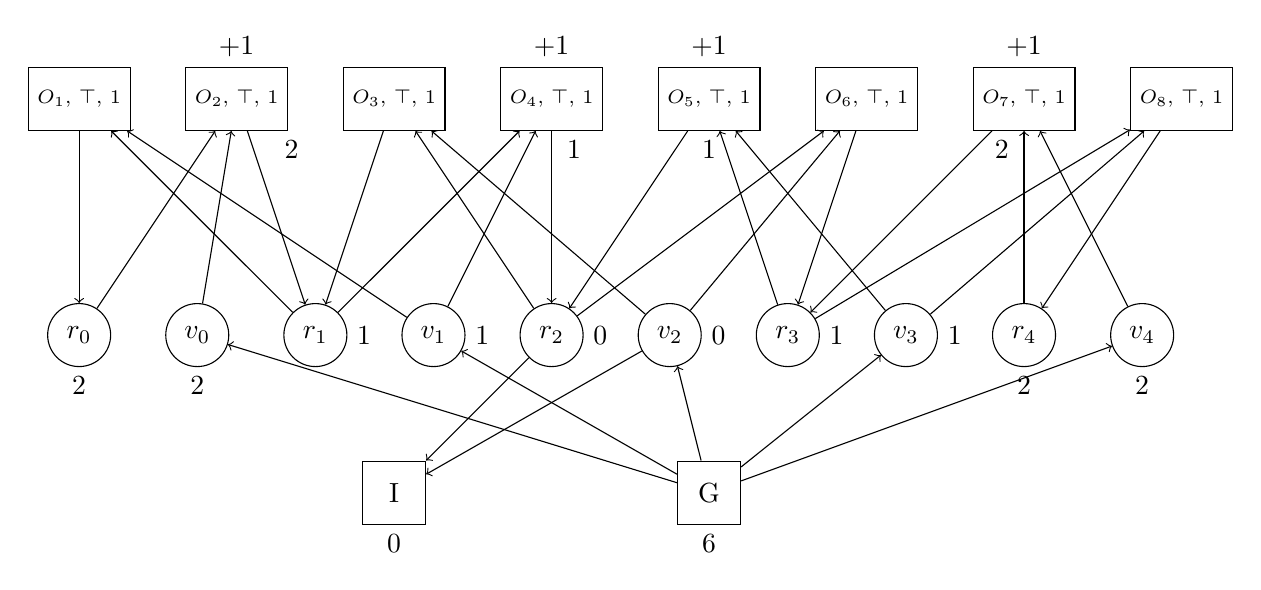
\begin{tikzpicture}[
        node distance=1.5cm and 1cm,
        mycirc/.style={draw, circle, minimum size=0.8cm}
        ]
    % Define styles
    \tikzstyle{square} = [draw, rectangle, minimum size=0.8cm]

    % Define operator nodes
    \node[square, font=\scriptsize] (O1) at (0, 6) {$O_1$, $\top$, 1};
    \node[square, font=\scriptsize, label=above:{+1}, label=-40:{2}] (O2) at (2, 6) {$O_2$, $\top$, 1};
    \node[square, font=\scriptsize] (O3) at (4, 6) {$O_3$, $\top$, 1};
    \node[square, font=\scriptsize, label=above:{+1}, label=-80:1] (O4) at (6, 6) {$O_4$, $\top$, 1};
    \node[square, font=\scriptsize, label=above:{+1}, label=below:{1}] (O5) at (8, 6) {$O_5$, $\top$, 1};
    \node[square, font=\scriptsize] (O6) at (10, 6) {$O_6$, $\top$, 1};
    \node[square, font=\scriptsize, label=above:{+1}, label=-100:{2}] (O7) at (12, 6) {$O_7$, $\top$, 1};
    \node[square, font=\scriptsize] (O8) at (14, 6) {$O_8$, $\top$, 1};

    % Define variable nodes
    \node[mycirc, label=below:{2}] (r0) at (0, 3) {$r_0$};
    \node[mycirc, label=below:{2}] (v0) at (1.5, 3) {$v_0$};
    \node[mycirc, label=right:{1}] (r1) at (3, 3) {$r_1$};
    \node[mycirc, label=right:{1}] (v1) at (4.5, 3) {$v_1$};
    \node[mycirc, label=right:{0}] (r2) at (6, 3) {$r_2$};
    \node[mycirc, label=right:{0}] (v2) at (7.5, 3) {$v_2$};
    \node[mycirc, label=right:{1}] (r3) at (9, 3) {$r_3$};
    \node[mycirc, label=right:{1}] (v3) at (10.5, 3) {$v_3$};
    \node[mycirc, label=below:{2}] (r4) at (12, 3) {$r_4$};
    \node[mycirc, label=below:{2}] (v4) at (13.5, 3) {$v_4$};

    % Define initial state and goal nodes
    \node[square, label=below:{0}] (I) at (4, 1) {I};
    \node[square, label=below:{6}] (G) at (8, 1) {G};

    % Draw edges from bottom from variable nodes to initial state
    \draw[->] (r2) -- (I);
    \draw[->] (v2) -- (I);

    % Draw edges from operator nodes to precondition nodes
    \draw[->] (O1) -- (r0);
    \draw[->] (O2) -- (r1);
    \draw[->] (O3) -- (r1);
    \draw[->] (O4) -- (r2);
    \draw[->] (O5) -- (r2);
    \draw[->] (O6) -- (r3);
    \draw[->] (O7) -- (r3);
    \draw[->] (O8) -- (r4);

    % Draw the edges from effect nodes to operator nodes
    \draw[->] (r1) -- (O1);
    \draw[->] (v1) -- (O1);
    \draw[->] (r0) -- (O2);
    \draw[->] (v0) -- (O2);
    \draw[->] (r2) -- (O3);
    \draw[->] (v2) -- (O3);
    \draw[->] (r1) -- (O4);
    \draw[->] (v1) -- (O4);
    \draw[->] (r3) -- (O5);
    \draw[->] (v3) -- (O5);
    \draw[->] (r2) -- (O6);
    \draw[->] (v2) -- (O6);
    \draw[->] (r4) -- (O7);
    \draw[->] (v4) -- (O7);
    \draw[->] (r3) -- (O8);
    \draw[->] (v3) -- (O8);

    % Draw edges from variables to goal
    \draw[->] (G) -- (v0);
    \draw[->] (G) -- (v1);
    \draw[->] (G) -- (v2);
    \draw[->] (G) -- (v3);
    \draw[->] (G) -- (v4);

\end{tikzpicture}

The value of $h^{add}(I)$ is 6.

\end{enumerate}

\end{titlepage}

\section*{Exercise 2}

For this exercise, we start by a) implementing an algorithm to compute the most conservative valuation
of an AND/OR graph and b) implementing an algorithm that constructs a relaxed task graph for a STRIPS 
task. We then run the \texttt{fast-downward} planner using our heuristic and compare it against blind
search on the \textit{castle} domain.
\vspace{5mm}

\begin{tabular}{|l|l|l|l|l|}
\hline
\multicolumn{1}{|c|}{} & \multicolumn{2}{|}{Number of Expansions} & \multicolumn{2}{c|}{Time (s)}\\
\cline{2-5}
\multicolumn{1}{|c|}{Instance} & Blind Search & Relaxed Task Graph & Blind Search & Relaxed Task Graph \\
\hline
castle 2-2-8 & 8 & 8 & 0.0014622 & 0.0013283 \\
\hline
castle 3-3-8 & 84 & 0.0022348 & 84 & 0.0029757 \\
\hline
castle 4-3-5 & 263 & 0.0034227 & 263 & 0.0071273 \\
\hline
castle 5-4-7 & 12 & 0.003974 & 6 & 0.0049379 \\
\hline
castle 5-4-9 & 7350 & 0.02681 & 7350 & 0.241813 \\
\hline
castle 5-4-10 & 0 & 0.0009523 & 0 & 0.0009358 \\
\hline
castle 6-4-7 & 24146 & 0.070907 & 24022 & 1.06481 \\
\hline
castle 7-5-4 & 3680953 & 12.537 & — & — \\
\hline
castle 8-5-9 & 4839625 & 16.9822 & — & — \\
\hline
castle 9-6-5 & 661 & 0.0117677 & 206 & 0.0594118 \\
\hline
castle 10-6-7 & — & — & — & — \\
\hline
castle 12-7-3 & 4585 & 0.0296206 & 2520 & 0.810473 \\
\hline
castle 16-9-1 & 22005 & 0.101019 & 4382 & 2.64418 \\
\hline
\end{tabular}

\end{document}
